\section{Solvers: from Bit Flips to Feasibility Projection}
\label{ch:solvers}

The QUBO formulation of the previous chapter defines a discrete energy
landscape over binary vectors, one bit per optional edge plus auxiliary
slack and flow variables. This chapter asks how that landscape can be
searched, and why the answer is less obvious than the phrase ``run an
annealer'' suggests. We proceed in three steps. First we describe a
conventional bit-level simulated annealer and the samplers against which
it is benchmarked. Second, we show that this entire family of methods
performs poorly on penalty-encoded constrained instances, and we trace
the failure to a structural property of the landscape rather than to
parameter tuning. Third, we describe the production solver, a projected
annealer whose moves live inside the feasible set, and we report its
measured accuracy against exact ground truth.

\subsection{A bit-level simulated annealer}
\label{sec:bit-sa}

Our reference annealer operates directly on the raw bit string. Each
variable of the QUBO, including edge bits, integer slack bits, and
directed flow bits, is a binary decision, and a move flips one of them.
A flip changes the energy by an amount computed incrementally from the
$Q$ matrix, so a single move costs $O(n)$ in the number of variables
rather than a full quadratic energy re-evaluation. The acceptance rule
is the standard Metropolis criterion: downhill moves are taken
unconditionally, and uphill moves of magnitude $\Delta E$ are accepted
with probability $\exp(-\Delta E / T)$.

The schedule is geometric cooling. Starting from an initial temperature
$T_0 = 10$, the temperature is multiplied by a cooling rate of $0.98$
after every two sweeps, where one sweep attempts one move per variable
on average, until a final temperature of $10^{-3}$ is reached. Two
extensions round out the design. First, with a configurable pair
probability, a move flips two bits simultaneously instead of one; this
helps the sampler traverse configurations in which two compensating
changes are neutral jointly but costly individually. Second, the
annealer accepts warm initial states, so a previously discovered
configuration can seed a new run rather than starting from a random
string.

Because the word ``effort'' is otherwise easy to game, the annealer
maintains an explicit counter of energy evaluations. Every comparison in
this chapter reports that counter, so that a solver which wins by doing
more work is visibly doing more work. This habit of honest accounting
matters here, because the production solver of
Section~\ref{sec:projected} does more work per move and we want that
visible rather than hidden.

\subsection{Why bit-level annealing fails on constrained QUBOs}
\label{sec:why-fails}

The failure mode is easy to state and hard to fix within the bit-flip
paradigm. In our encoding, hard constraints are enforced by penalty
terms whose weights, between $100$ and $500$, are chosen to dominate the
soft objective: the utility of a single edge is at most about $1$, so
breaking one constraint costs at least one hundred times more than any
single edge can ever be worth. The intended consequence is that any
optimizer which minimizes total energy will respect the constraints. The
unintended consequence is that the energy landscape becomes a set of
deep, narrow valleys separated by enormous barriers.

Consider a Metropolis sampler sitting in a feasible configuration and
contemplating a single bit flip. Almost every flip that touches a
constraint variable produces a state that violates a constraint, with an
energy increase of at least $100$. At temperature $T = 1$, such a move
is accepted with probability below $e^{-100}$, which is zero for all
practical purposes. The sampler is therefore confined to the feasible
region it started in, able to leave it only at the high temperatures of
the early schedule, when acceptance is indiscriminate and no useful
signal is retained. Cooling then strands it in whichever valley it
happened to occupy. Random restarts do not rescue the method: starting
from uniformly random bit strings, the bit-level annealer returned an
infeasible final state in 19 of 25 test instances. The sampler could not
even find its way back into the feasible region, let alone optimize
within it.

We emphasize that this is not a complaint about a particular
implementation. Penalty-encoded constraints create, by construction,
barriers that single-bit moves cannot cross at useful temperatures.
Stronger cooling schedules, more sweeps, or pair moves shift the numbers
by a few percentage points but do not address the geometry.

\subsection{Sampler benchmark on the real Q matrices}
\label{sec:sampler-bench}

To quantify the claim, we benchmarked four samplers on the actual $Q$
matrices produced by our encoding for 25 representative instances, with
ground truth defined two ways. For each instance, the exact optimum of
the constrained problem was obtained by complete enumeration of the
optional-edge subsets, and the exact minimum of the encoded QUBO was
obtained by a linearized exact solve with CBC, which converts each
quadratic term into an auxiliary variable and proves optimality with a
branch-and-bound search. The two agree wherever both are computable;
the CBC solve is the ground truth for what a sampler \emph{should}
return.

Table~\ref{tab:sampler-results} summarizes the outcome. The local
bit-level annealer reaches the exact optimum in 56\% of instances.
D-Wave's \code{neal} sampler, a mature open-source simulated annealing
implementation, reaches 60\%. Tabu search reaches 64\%, the best of the
four, and simulated quantum annealing through OpenJij reaches 48\%, the
worst. No sampler clears two thirds. Figure~\ref{fig:sampler-rates}
shows the same numbers against the exact reference at 100\%.

\begin{table}[t]
  \centering
  \caption{Schedules and defaults of the solvers compared in this
  chapter. The bit-level annealer, \code{neal}, tabu, and simulated
  quantum annealing (SQA) all operate on the raw bit string of the
  encoded QUBO. The projected annealer operates on feasible edge sets;
  its temperature range is lower because its moves change the soft
  objective only.}
  \label{tab:solver-schedules}
  \small
  \begin{tabular}{lccccc}
    \toprule
    Solver & $T_{\mathrm{init}}$ & $T_{\mathrm{final}}$ &
    Cooling & Steps per $T$ & Restarts \\
    \midrule
    Bit-level SA & 10 & $10^{-3}$ & 0.98 & 2 sweeps & 1 (warm optional) \\
    \code{neal} & \multicolumn{3}{c}{default \code{beta\_range}} &
    default sweeps & 1 \\
    Tabu search & \multicolumn{3}{c}{n/a (tenure-based)} &
    default iterations & 1 \\
    SQA (OpenJij) & \multicolumn{3}{c}{default transverse-field schedule}
    & default sweeps & 1 \\
    Projected annealer & 1.0 & $10^{-2}$ & 0.998 & 4 & 5 \\
    \bottomrule
  \end{tabular}
\end{table}

\begin{table}[t]
  \centering
  \caption{Exact-solution rates on 25 instances with enumerated ground
  truth. ``Infeasible'' counts runs whose returned bit string violates
  at least one constraint. The projected annealer is excluded from this
  comparison by design; see Section~\ref{sec:projected-honesty}.}
  \label{tab:sampler-results}
  \small
  \begin{tabular}{lcc}
    \toprule
    Sampler & Exact rate & Returned infeasible \\
    \midrule
    Bit-level SA (ours) & 56\% & 19 of 25 (random restarts) \\
    \code{neal} & 60\% & n/a \\
    Tabu search & 64\% & n/a \\
    SQA (OpenJij) & 48\% & n/a \\
    \midrule
    Exact linearized solve (CBC) & 100\% (reference) & 0 \\
    \bottomrule
  \end{tabular}
\end{table}

\begin{figure}[t]
  \centering
  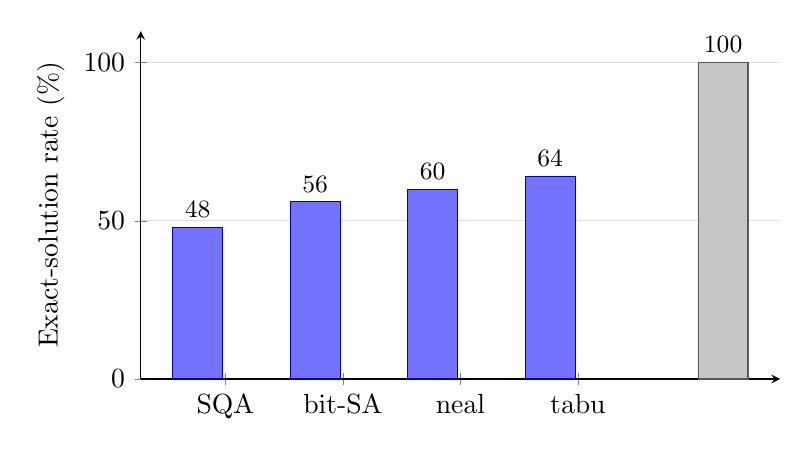
\begin{tikzpicture}
    \begin{axis}[
      ybar,
      width=0.8\textwidth,
      height=6cm,
      bar width=18pt,
      ymin=0, ymax=110,
      ylabel={Exact-solution rate (\%)},
      symbolic x coords={SQA, bit-SA, neal, tabu, exact (CBC)},
      xtick=data,
      nodes near coords,
      nodes near coords align={vertical},
      every node near coord/.append style={font=\small},
      ymajorgrids=true,
      grid style={gray!25},
      axis lines=left,
      enlarge x limits=0.18,
    ]
      \addplot[fill=blue!55, draw=blue!70!black] coordinates
        {(SQA,48) (bit-SA,56) (neal,60) (tabu,64)};
      \addplot[fill=gray!45, draw=gray!70!black] coordinates
        {(exact (CBC),100)};
    \end{axis}
  \end{tikzpicture}
  \caption{Exact-solution rates of four samplers on 25 QUBO instances
  derived from our encoding. The gray bar is the exact linearized CBC
  solve at 100\%, which defines the ground truth against which all
  sampler rates are measured; it is a reference, not a competitor.}
  \label{fig:sampler-rates}
\end{figure}

Two conclusions follow. First, the weakness is shared across
implementations and paradigms: classical annealing, tabu search, and
simulated quantum annealing all struggle, which supports the geometric
explanation of Section~\ref{sec:why-fails} over any
implementation-specific one. Second, the Q matrix itself is not at
fault, because the exact linearized solve of that same matrix recovers
the true optimum every time. The encoding is a faithful specification;
generic samplers are simply poor at searching it.

\subsection{The production solver: feasibility-projected edge annealing}
\label{sec:projected}

The production solver changes the search space rather than the search
algorithm. Instead of annealing over raw bit strings and hoping to land
inside the feasible region, it anneals directly over the set of feasible
edge subsets. A state is a set of kept edges together with the slack and
flow assignments that certify its feasibility; the energy of a state is
exactly the QUBO energy evaluated at that certificate. On the feasible
manifold the penalty terms vanish identically, so the energy reduces to
the soft objective, and the sampler never wastes a single evaluation on
a constraint violation.

Two move types generate candidates, as illustrated in
Figure~\ref{fig:moves}. A \emph{toggle} adds or removes one optional
edge. A \emph{swap} exchanges two edges, one in and one out, which
allows the solver to reallocate budget or degree capacity between parts
of the graph in a single step. Not every candidate is feasible: adding
an edge can exceed a degree cap or the global budget, and removing one
can disconnect a required node from the root. Each candidate is
therefore passed through a projection step, an exact repair procedure
that recomputes the integer slack variables and rebuilds a spanning-tree
flow certifying connectivity. If the repair succeeds, the repaired state
is the candidate actually scored; if no feasible repair exists, the move
is rejected outright. Projection is deterministic and exact, so the
solver's trajectory never leaves the feasible set.

\begin{figure}[t]
  \centering
  \begin{tikzpicture}[
    node distance=9mm and 11mm,
    vertex/.style={circle, draw=black!70, fill=blue!12, inner sep=1.6pt,
      minimum size=5.2mm, font=\small},
    kept/.style={draw=blue!70!black, very thick},
    gone/.style={draw=red!75!black, thick, dashed},
    added/.style={draw=green!55!black, very thick},
    panel/.style={draw=black!40, rounded corners=2pt, inner sep=4pt},
    lbl/.style={font=\small\itshape, text=black!70},
  ]
    % toggle panel
    \begin{scope}[local bounding box=toggle]
      \node[vertex] (t1) {1};
      \node[vertex, right=of t1] (t2) {2};
      \node[vertex, below=of t1] (t3) {3};
      \node[vertex, right=of t3] (t4) {4};
      \draw[kept] (t1) -- (t2);
      \draw[kept] (t1) -- (t3);
      \draw[kept] (t2) -- (t4);
      \draw[gone] (t3) -- (t4);
      \node[lbl, below=3mm of t3, xshift=8mm] {toggle: drop edge $(3,4)$};
    \end{scope}
    % swap panel
    \begin{scope}[local bounding box=swap, xshift=5.6cm]
      \node[vertex] (s1) {1};
      \node[vertex, right=of s1] (s2) {2};
      \node[vertex, below=of s1] (s3) {3};
      \node[vertex, right=of s3] (s4) {4};
      \draw[kept] (s1) -- (s2);
      \draw[kept] (s1) -- (s3);
      \draw[gone] (s2) -- (s4);
      \draw[added] (s3) -- (s4);
      \node[lbl, below=3mm of s3, xshift=8mm]
        {swap: out $(2,4)$, in $(3,4)$};
    \end{scope}
    % projection panel
    \begin{scope}[local bounding box=proj, xshift=11.2cm]
      \node[vertex] (p1) {1};
      \node[vertex, right=of p1] (p2) {2};
      \node[vertex, below=of p1] (p3) {3};
      \node[vertex, right=of p3] (p4) {4};
      \draw[kept] (p1) -- (p2);
      \draw[kept] (p1) -- (p3);
      \draw[added] (p3) -- (p4);
      \node[lbl, below=3mm of p3, xshift=8mm]
        {repair: slack + flow rebuilt};
    \end{scope}
    % arrows between panels
    \draw[-{Stealth[length=3mm]}, thick, black!60]
      (toggle.east) -- (swap.west);
    \draw[-{Stealth[length=3mm]}, thick, black!60]
      (swap.east) -- (proj.west);
    \begin{scope}[on background layer]
      \node[panel, fit=(toggle)] {};
      \node[panel, fit=(swap)] {};
      \node[panel, fit=(proj)] {};
    \end{scope}
  \end{tikzpicture}
  \caption{The move set of the projected annealer. Solid blue edges are
  kept, the dashed red edge is removed, and the green edge is added. A
  toggle changes one optional edge; a swap exchanges two. The right
  panel shows the projection step: after the move, integer slack
  variables and a spanning-tree flow from the root are recomputed
  exactly, and the candidate is accepted only if the repair succeeds.}
  \label{fig:moves}
\end{figure}

Restarts require care, for the same geometric reason that defeats
bit-level annealing. Greedy edge-by-edge growth, adding the
highest-utility edge that keeps the partial solution feasible, cannot
cross the infeasible prefix states that the connectivity constraint
creates: a cheap subtree can be constructed that is locally feasible yet
admits no feasible completion within budget. Restart states are
therefore generated as degree-cap-aware random spanning trees, sampled
so that every partial state is a tree that already respects the degree
limits, and then completed with any budget-feasible extra edges. This
guarantees that every restart begins inside the feasible manifold with a
diverse geometry.

After cooling, a deterministic polish drives the incumbent to a local
fixpoint. The polish alternates a pass of all single toggles with a pass
of all pairwise swaps, accepting every strict improvement, until neither
pass finds one. The polish is cheap relative to the anneal and removes
the residual noise that a finite temperature schedule leaves behind.

It is worth being precise about what the QUBO has become in this design.
The QUBO remains the specification of the problem: the energy function,
the constraint weights, and the feasibility test are all defined by it,
and the $Q$ matrix is still exported for hardware backends, so a quantum
or dedicated annealing device can be substituted for the classical
sampler without touching the formulation. The projected annealer is best
understood as a classical sampler that exploits the known structure of
the penalty terms to restrict itself to the subspace where those terms
are zero.

\subsection{Defaults, measured cost, and accuracy}
\label{sec:projected-results}

The production defaults are deliberately mild, because the feasible
manifold is a friendlier landscape than the raw bit space. The initial
temperature is $1.0$, the final temperature is $10^{-2}$, the cooling
rate is $0.998$, and each temperature holds for four steps. Toggles and
swaps are proposed with equal probability $0.5$. Five restarts are
drawn from the random spanning-tree generator, and in the live system
the previous cycle's kept edges are supplied as a warm start, so that
successive cycles refine an incumbent rather than restarting from
scratch.

Measured on the benchmark instances, a solve performs about $2.4 \times
10^{4}$ energy evaluations and takes about $2.1$ seconds of wall time on
commodity hardware. The accuracy numbers are the following.

\begin{itemize}
  \item \textbf{Small instances.} On the 25 instances with enumerated
  ground truth, the projected annealer returns the exact optimum in
  100\% of cases, against 56\% to 64\% for the raw-space samplers of
  Table~\ref{tab:sampler-results}.
  \item \textbf{Larger instances.} On 20 larger instances where
  enumeration is infeasible and ground truth comes from the exact MILP
  solve of the original constrained problem, the projected annealer is
  exact in 95\% of cases, with a mean true optimality gap of $7 \times
  10^{-5}$ and a worst-case gap of $1.4 \times 10^{-3}$.
  \item \textbf{Robustness.} Across a sensitivity sweep that perturbs
  the initial and final temperatures, the cooling rate, the restart
  count, the penalty scales, and the pair probability, the solver
  remains exact in 87\% of configurations. Accuracy degrades gracefully
  rather than catastrophically when the schedule is mistuned.
\end{itemize}

\subsection{An honest framing}
\label{sec:projected-honesty}

The projected annealer is not entered into the sampler comparison of
Section~\ref{sec:sampler-bench}, and we want the reason on record. Its
move set is richer than what a generic sampler is permitted: it exploits
domain knowledge, namely the structure of the constraint set, the
meaning of the slack variables, and the availability of an exact repair
procedure, that a hardware annealer or a black-box sampler acting on a
raw $Q$ matrix does not have. Comparing it against \code{neal}, tabu, or
OpenJij on equal footing would conflate two different questions: how
well generic samplers search penalty-encoded QUBOs, and how well a
structure-aware classical algorithm solves the underlying constrained
problem. The first question is the scientifically interesting one for
assessing quantum and quantum-inspired hardware, and it is answered by
Table~\ref{tab:sampler-results}. The projected annealer is therefore
reported as an engineering note: it is the solver the deployed system
actually uses, and its near-exact results establish that the QUBO
formulation itself, not any solver, is the binding constraint on
end-to-end performance. Where a classical exact optimum is affordable,
the MILP solve remains both faster and provably optimal, and the
evaluation chapter makes that comparison directly.
